\chapter{Introduzione}
\section{UAV}
\begin{figure}[h]
    \centering
    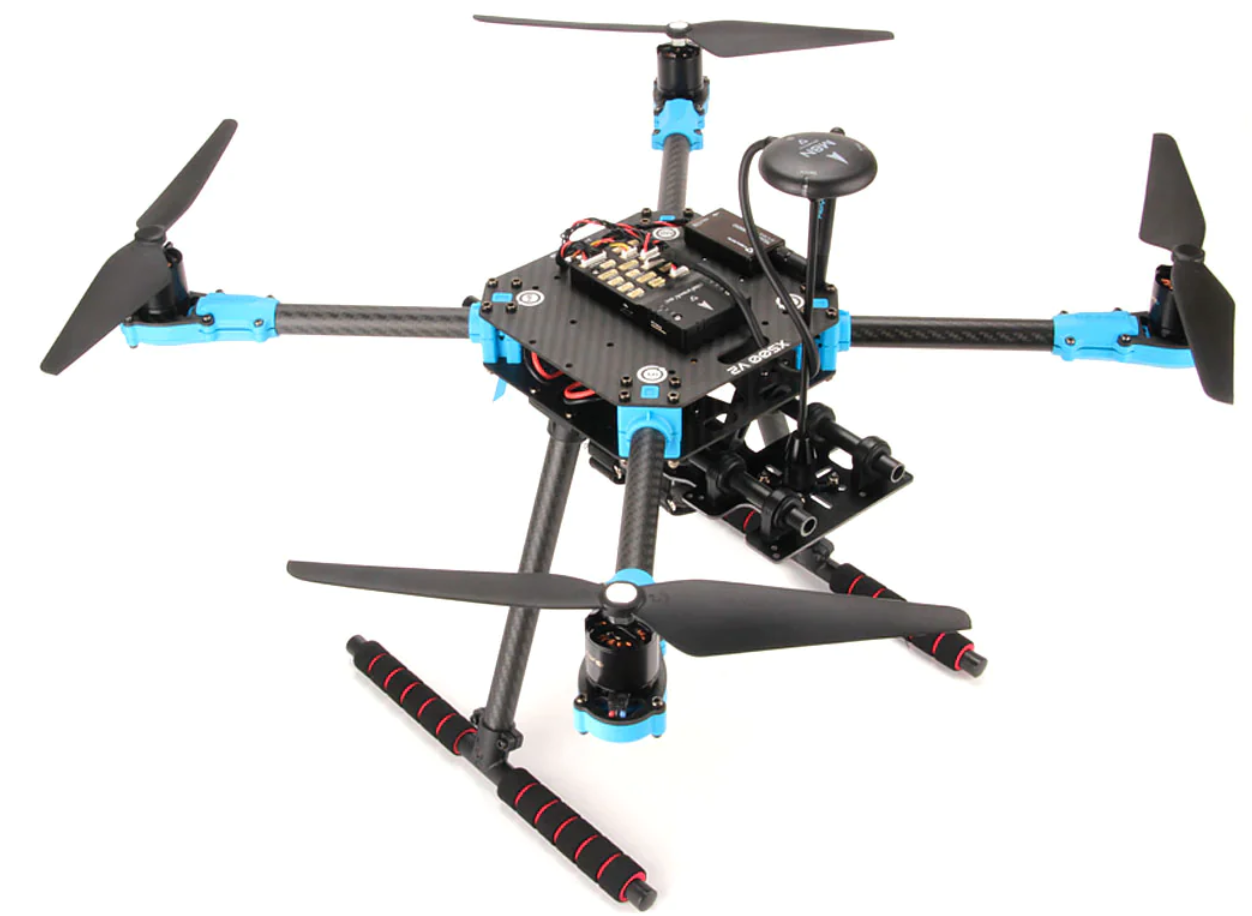
\includegraphics[width=0.7\linewidth]{files/drone.png}
    \caption{Quadricottero Holybro}
    \label{fig:enter-label}
\end{figure}
Un veicolo aereo senza equipaggio (UAV), noto anche come drone, è un aeromobile autonomo che opera senza la presenza umana a bordo. Attualmente, gli UAV sono ampiamente utilizzati in svariate applicazioni, tra cui la fotografia aerea, l'agricoltura di precisione, il monitoraggio ambientale, la sorveglianza e il trasporto.
\\~\\
Dal punto di vista tecnico, il controllo di un drone coinvolge diverse componenti hardware e software:
\subsubsection*{Hardware:}
\begin{itemize}
    \item \textbf{Microprocessore Primario:} Il cuore del sistema di controllo, responsabile dell'esecuzione delle istruzioni di volo.
    \item \textbf{Processore Secondario (Failsafe):} Garantisce la sicurezza del volo intervenendo in situazioni di emergenza o malfunzionamenti del sistema principale.
    \item \textbf{Attuatori:} Include regolatori di velocità elettronici (ESCs) che gestiscono la potenza fornita ai motori, controllando così il movimento del drone.
    \item \textbf{Sensori a Gradi di Libertà (DOF):} Per esempio, giroscopi e accelerometri a 3 assi (6DOF) per monitorare l'orientamento e il movimento del drone. Sensori a 11DOF possono includere barometro, bussola e GPS per una maggiore precisione.
\end{itemize}

\subsubsection*{Software:}
\begin{itemize}
    \item \textbf{Autopilota o Stack di Volo:} Responsabile dell'esecuzione delle missioni di volo in modo autonomo o in risposta a input remoti. Gestisce la stabilizzazione, il controllo degli attuatori e la navigazione.
    \item \textbf{Firmware:} Il software incorporato che gestisce il codice macchina, l'esecuzione del processore e l'accesso alla memoria. Deve essere altamente affidabile e efficiente.
    \item \textbf{Middleware:} Gestisce la comunicazione tra i vari componenti del sistema, facilitando il flusso di dati e comandi tra sensori, attuatori e autopilota.
    \item \textbf{Sistema Operativo:} Ad esempio, ROS (Robot Operating System), Nuttx o Linux, fornisce un ambiente operativo che consente di eseguire complesse operazioni di controllo, pianificazione di volo e acquisizione dati in tempo reale.
\end{itemize}
Gli UAV operano in tempo reale, richiedendo una rapida elaborazione dei dati sensoriali. L'integrazione efficiente tra hardware e software è essenziale per garantire il controllo stabile e sicuro del drone durante tutte le fasi della missione.
\\~\\
L'evoluzione dei sistemi integrati, come i veicoli senza pilota, con unità di controllo e vari sensori complessi, ha reso i tradizionali test su macchine reali costosi e complessi, data la presenza di molteplici sensori come IMU, georadar e termocamere. L'impiego del concetto "Hardware-In-The-Loop" (HITL) emerge come soluzione strategica. Questa metodologia consente di condurre test completi senza la necessità di utilizzare direttamente sul campo un prodotto finale assemblato, affrontando la sfida delle grandi mole di dati e riducendo i costi associati ai test in tempo e spazio reali.
\section{Hardware-In-The-Loop (HITL)}
Il termine "Hardware-In-The-Loop" (HITL) si riferisce a una serie di metodologie utilizzate per verificare il funzionamento di dispositivi hardware connessi a una piattaforma di simulazione in grado di emulare il comportamento del sistema reale. Questo approccio consente di testare gli algoritmi di controllo durante la fase di progettazione, eliminando la necessità di attendere la disponibilità del prodotto finale e riducendo tempi e costi associati ai test fisici.
\\~\\
Grazie all'utilizzo dell'HITL è possibile:
\begin{itemize}
    \item Creare e simulare una rappresentazione virtuale dei componenti fisici;
    \item Eseguire algoritmi di controllo sulla simulazione, permettendo l'interazione con il dispositivo fisico attraverso canali di Input/Output.
\end{itemize}
Questa metodologia risulta particolarmente vantaggiosa in situazioni in cui testare l'algoritmo di controllo direttamente sul sistema fisico sarebbe costoso e/o pericoloso. 
\section{Obiettivo del Progetto}
Il progetto mira a stabilire una connessione Hardware-In-The-Loop (HITL) tra PX4 ed il MATLAB UAV Toolbox, sfruttando le librerie disponibili per:
\begin{itemize}
    \item Log dei segnali del Flight Controller e del Plant Model
    \item Simulazione di guasti alle componenti di attuazione e sensoristica
    \item Sviluppo di algoritmi di rilevamento guasti
\end{itemize}
L'accesso alle misure sensoriali, combinato con la capacità di simulare guasti, fornisce la base per lo sviluppo di algoritmi di diagnosi o di controllo tollerante ai guasti.
\\~\\
Il percorso del progetto prevede le seguenti fasi indicative:
\begin{itemize}
    \item Installazione e configurazione del software di simulazione con il modello del drone.
    \item Analisi del simulatore per identificare e comprendere le librerie disponibili.
    \item Implementazione della connessione HITL tra PX4 e MATLAB.
    \item Simulazione di un guasto e acquisizione dei dati sensoriali.
    \item Valutazione delle modalità per modificare il Flight Controller
    \item Sviluppare algoritmi di rilevamento guasti attraverso l'integrazione con il MATLAB UAV Toolbox.
\end{itemize}
L'obiettivo finale è ottenere una piattaforma funzionale che consenta di esplorare e implementare algoritmi avanzati di controllo e diagnostica per droni, migliorando la comprensione e la gestione dei guasti in un contesto di volo.